%\documentclass[10pt, conference, compsocconf]{IEEEtran}
\documentclass[10pt, conference, compsocconf]{IEEEtran}
\usepackage{color}
\usepackage{supertabular}
\usepackage{graphicx}
\usepackage{flushend}
\usepackage{cite}
\usepackage{subfigure}
\usepackage{comment}
\usepackage[cmex10]{amsmath}


\bibliographystyle{IEEEtran}

\begin{document}

\newcommand {\xtq}[1] {\begin{color}{red}{[XTQ : #1]}\end{color}}
%start title
%\title{Studies of Cloud Based Burst Buffers to Burst Data Intensive Application on
%the Cloud}
\title{Explorations of Cloud-based Burst Buffers for I/O Acceleration}%Data Caching}%Data Intensive
% Applications }

\author{
\IEEEauthorblockN{Tianqi Xu}
	\IEEEauthorblockA{Dept. of Mathematical\\and Computing Sciences\\
		Tokyo Institute of Technology\\
		2-12-1-W8-33, Ohokayama,\\
		Meguro-ku, Tokyo 152-8552 Japan\\
	Email: belldandyxtq@gmail.com}
	\and
	\IEEEauthorblockN{Kento Sato}
	\IEEEauthorblockA{Center for Applied Scientific Computing\\
		Lawrence Livermore National Laboratory\\
		Livermore, CA 94551 USA\\
	Email: kento@llnl.gov}
	\and
	\IEEEauthorblockN{Satoshi Matsuoka}
	\IEEEauthorblockA{Global Scientific \\Information and Computing Center\\
		Tokyo Institute of Technology\\
		2-12-1-W8-33, Ohokayama,\\
		Meguro-ku, Tokyo 152-8552 Japan\\
	Email: matsu@is.titech.ac.jp}
}

\maketitle

%start abstract
\begin{abstract}
Cloud offers high computational resources, strong scalability, as well as easy to access. 
Such cloud environment offers these who have limited local computational resources a opportunity to
run large scale applications.
Current data intensive large scale applications generate TB intermediate data shared among hundreds
of compute nodes, so the shared storage throughput becomes critical part.
However compare to the throughput in HPC system, the shared storage
system in cloud environment can only achieve a quite low I/O throughput, becoming the
performance bottleneck for data intensive applications.
Furthermore, according to normal cloud pay-as-you-go pricing, longer execution time means more you
should pay.
In this paper, we propose a cloud based burst
buffer system as a new tier in cloud storage system to absorb I/O request.
We use several nodes as a burst buffer nodes, take advantage of high throughput inside cloud to
buffer application I/O data.
We implemented a prototype of our proposal architecture, evaluated in Amazon EC2/S3(one of the most
common public cloud today).
We shows our system can achieve a significant improvement in I/O throughput for shared storage
in cloud computing through experimental and simulation evaluation.
\end{abstract}

%start key word
\begin{IEEEkeywords}
	cloud computing, burst buffer
\end{IEEEkeywords}

\IEEEpeerreviewmaketitle

%section I
\section{Introduction}
\label{sec:introduction}
% Kento: Growing focus ``does not'' allows users to run ...
% A growing focus on cloud computing for its high scalability as well as high computational
% resources, for example, Amazon provided a high performance computing instance allows user to run
% complex science, engineering, and business applications on these instances with a high bandwidth low latency
% network, and high compute capabilities.
% Cloud provide a fast setup, usually cloud instances can set up in a few
% minutes, this make the on-demand usage available. 
% Such cloud environment is suitable for large scale
% computation, by using cloud users don't need a large scale supercomputer and
% only need to pay what they run, instead of dealing with expensive hardware, software and machine maintenance.
% These characteristics make cloud very attractive to large-scale applications.
Cloud have been gathering attention of application developers because
of its elasticity. With the elasticity, the users enjoy virtually unlimited
computational resources on the fly, and pay the cost depending on the usage.
In addition, recent clouds also provides computational resources for high
performance computing
\cite{AMAZON_AWS,Azure,IBM_public_cloud,oracle_cloud,hp_cloud}.
The computational power and the scalability enable the users to run high
performance scientific applications faster than ever.
For example, Amazon EC2 provides HPC instances with high bandwidth networks,
SSD-embedded I/O subsystems and GPU accelerators\cite{AWS_HPC}.
These characteristics make cloud computing more attractive to large scale
scientific applications.
\par
% Large-scale applications often require high I/O
% throughput and data sharing between different nodes, different work flow and even different jobs.
% In such cases, applications require not only high bandwidth network as well as a high throughput
% shared storage in order to share data between different nodes, different work flow or difference
% jobs.
% Applications like Montage\cite{montage} Pov Ray\cite{povray} generate huge size of intermediate file
% need to be shared between different nodes in different work flow.
% Such applications are now running majorly on high performance computing system like supercomputers,
% with a GB/s level shared storage as well as high interconnection network.
% Furthermore, large scale applications require for a large amount of compute node as well as a
% running time from several hours to several days, machine failure is Inevitable and checkpoint will be required to enable
% fast recovery from machine failure\cite{checkpointing}, in order to make a timely checkpoint, a
% fast global shared storage is indispensable.
% 
% However, in current cloud environment, the global shared storage can not meet the demand.
% For example, in Amazon public cloud system, there are a famous shared storage called \emph{Amazon
% Simple Storage Service} (Amazon S3)\cite{AMAZON_AWS}, however compared to the throughput of shared
% storage system in high performance computing system, Amazon S3 can only achieve a extremely low throughput,
% as well as has a high latency, since storage machine in Amazon S3 are geographically distributed and connected via Internet.
% Also it is difficult to build each compute center a reasonable size data center, since it cannot
% achieve a high utilization of storage system.

However, if we execute \emph{data intensive workloads}, such as big data
analysis and checkpointing for visualization or fault tolerance, on a cloud environment, the
users suffer from the prolonged execution time and the cost because of the low
throughput to shared storage and the data intensive workloads.
For example, cloud-based shared storage, Amazon Simple Storage Service (Amazon
S3), provides only a few hundreds MB/s of throughput because instances
in Amazon EC2 is connected to Amazon S3 via Internet.
As demands for higher I/O throughput grow, 
current cloud environments cannot provide enough I/O performance for 
\emph{data intensive workloads}.
Thus, improvement of I/O performance in clouds is critical to accelerate such
\emph{data intensive workloads}.
\par
% In order to solve such problem, we propose a cloud based burst buffer system. Burst buffer system
% has been proposed as a new tier in the storage hierarchy to hide the low bandwidth and high latency
% of the shared file system by allocate several local nodes as a burst buffer nodes to absorb the I/O
% request from applications, our proposal system using such burst buffer system and take advantage of
% high throughput, low latency interconnection network inside cloud environment, make some of compute
% nodes as a I/O burst buffer nodes to buffer I/O data and bursting I/O sensitive applications in cloud environment.
% To validate effectiveness of burst buffers in cloud, we implemented a prototype of our
% proposal system and evaluated on real public cloud environment,
% % as well as simulated with several applications.\xtq{we e}
% We achieved 3 times speed up on reading as well as 4 times speed up on writing with 8 I/O nodes, and
% achieved a up to 4 times speed up on execution of data intensive applications from simulation.
In order to solve the problem, we propose a cloud-based burst buffer system.
Burst buffers have been proposed as a new tier of storage in the storage
hierarchy in order to provide higher I/O throughput for shared storage by
absorbing bursty I/O requests from applications running on supercomputers
\cite{on_the_role_of_burst_buffers}.
Because most of HPC applications have data access
locality, if we cache the data, which is accessed in near future, on the burst
buffers, we can accelerate the access performance to the data
\cite{montage,povray}.
In addition, if we apply burst buffers to clouds, we can build on-demand burst
buffers by taking advantage of the elasticity in clouds. 
%\kento{local storage use ? in-memory}
To explore the effectiveness of burst buffers in clouds, 
we implement a prototype of a cloud-based burst buffer system, and models the
system to estimate execution time of data intensive applications.
Our experimental results using Amazon EC2 shows that we achieve 3 times of
improvement in read throughput, and 4 times in write throughput with 8 nodes of
burst buffers. Our simulation based on the model shows that we can
improve execution time of real data intensive applications by 2.5 times in
execution time.
\par


Our contributions can be summarized as following:
\begin{itemize}
	\item A cloud-based burst buffer system accelerating data intensive
	workloads in cloud environments;
	\item Models estimating I/O throughput in a real cloud environment
	\item Improvement of I/O performance by using our cloud-based burst buffer
	system in Amazon EC2;
    \item Quantitative evaluations targeting real environments where
    multiple real applications run, and access to the cloud-based burst
    buffers;
\end{itemize}
%2
\par
The rest of this paper is organized as follows. 
In Section \ref{sec:background}, we describe the background and the motivation.
Then, we describe the details of our cloud-based burst buffer system
implementation in Section \ref{sec:implementation}, and the modeling in Section
\ref{sec:modeling}. Next, in Section \ref{sec:evaluation}, we present our experimental results of the cloud-based burst buffer system.
Finally, we describe related work in Section \ref{sec:related work}, and
conclusion in Section \ref{sec:conclusion}.


%section II
%to do
\section{Background and Motivation}
\label{sec:background}
If we execute data intensive workloads in clouds, the performance is
expected to be unacceptable because I/O performance of shared storage in
clouds are fairly slow (in Section \ref{ssec:IO_performance_in_clouds}). 
However, our analysis of data intensive workloads on HPC systems, we found
that a number of applications have temporal I/O locality (in Section
\ref{ssec:data_access_locality}). These I/O workloads can be accelerated even on
clouds where shared storage performance is low (in Section
\ref{ssec:network_s3}) if we use our cloud-based burst buffer system works as an
\emph{on-demand remote cache space}. 


\begin{comment}
\subsection{Cloud Computing}
\begin{figure}
\centering
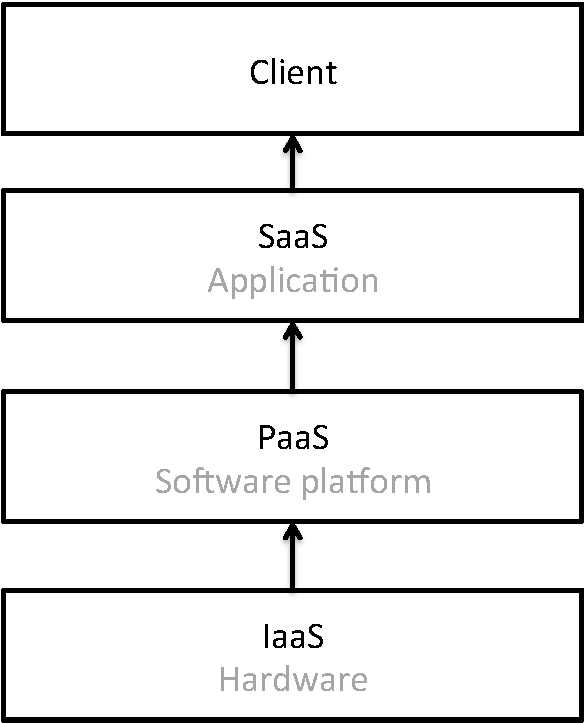
\includegraphics[width=4cm]{img/cloud_models.pdf}
\caption{the relationship of different cloud models}
\label{background:cloud models}
\end{figure}

Cloud computing refers to a model that cloud vendors provide user IT resources and charge them for
the resources they used.
Cloud vendors can offer hardware resources including CPU, memory, hard disk, network and software
resources OS, software suits and applications.
Cloud computing majorly can be classified into following three kinds of models:
\begin{enumerate}
  \item Infrastructure as a service (IaaS): cloud vendors provide only raw machines(physical or
  virtual machine), user need to set up the whole software environment including OS.
  \item Platform as a service (PaaS): in this model, cloud vendors provide
  hardware as well as software platform. Users can use it as a common computer and run applications on the platform.
  Amazon EC2 provides PaaS.
  \item Software as a service (SaaS): Cloud vendors provide a certain applications. Users don't need
  to configure the software themselves.
\end{enumerate}
The relationship of different cloud models can be shown as Figure~.\ref{background:cloud models}

Cloud computing can have following benefits:
\begin{itemize}
  \item Users don't need to care about the machine placement and maintenance.
  \item Users don't need a large number of machines to meet a temporally request peek and idle for
  the other time, Since cloud instances can set up in a few minutes when the request peek occurs.
  \item Users don't need to pay for expensive hardware and software, they just need to pay for what
  they used.
\end{itemize}
\end{comment}
\subsection{I/O Performance in Cloud Storage}
\label{ssec:IO_performance_in_clouds}

% \kento{There is no topic sentence in this subsection. Why did you write this
% Subection ? why do you compare  Interconnection Network vs. Shared Storage}
% In public cloud system, although shared storage cannot achieve a high performance, the
% interconnection network between compute nodes usually has a high bandwidth.
% Our proposal system takes advantage of high throughput of interconnection network between compute
% nodes inside cloud system to burst I/O throughput.
% In order to show the difference of throughput between Amazon S3 and interconnection network between
% compute nodes.
% First we measured the sequential I/O performance of Amazon S3, we measured read and write throughput
% with different size of compute nodes, and we also measured the two I/O pattern performance which
% will compute nodes shared the same file and each compute nodes access to different file.
% Figure~\ref{background:amazon s3 throughput} shows the result, we can see that compare to modern parallel file systems in HPC systems, for example TSUBAME lustre can achieve 6-8GB/s\cite{checkpointing}
%  Amazon S3 cannot achieve a high throughput, and the value is
% quite unstable.
% Many previous studies also measured the I/O throughput in clouds
% \cite{Chiba,Transactions_a_la_carte, Interactive_Use_of_Cloud_Services,Amazon_S3_for_Science_Grids,
% anevaluation} and got a similar result.
% \kento{Because you already evaluated S3 performance, I do not think this
% paragraph is necessary. Instead, please use these sentences to support your
% results, and show the results are consistent to evaluations done by others}
%  
% However, when we look at the point to point communication throughput between two compute nodes
% inside Amazon EC2,
% We measure this interconnection network by using Iperf [14].
% \kento{What does the ``inside'' mean ? please describe what did you measure}
% Figure.~\ref{background:amazon throughput} shows a comparison of Amazon Interconnection Network
% throughput and Amazon S3 throughput, although we only show the result up to 8 pairs of nodes
% \kento{Because you did not describe how to measure the performance,
% ``pairs'' is not unknown}, each node achieved only 135MB/s (1GBit/s), the
% influence between nodes is extremely small, figure shows a perfect linear line also a strong scalability.
% \kento{It's too detailed. And Should be mentioned before showing results}.
% When we running the
% benchmark, many other users were also running applications on Amazon, so we can assume that highest
% throughput 1GB/s (8Gbit/s) shown in Figure.~\ref{background:amazon throughput} is not the
% maximum bandwidth of interconnection network in Amazon EC2 \kento{Why do you
% mention this ? If you want to say ``this results is not trustful because other
% applications were running'', please remove this figure and this subsection.
% Instead, you should mention ``Even with other applications are running, the
% performance is still better than S3'' . But, in fat tree topology, almost peak
% throughput can be achieved even if other applications are running like in
% TSUBAME. So I do not think your expectation is true}.
% As Figure.~\ref{background:amazon throughput} shows, Interconnection Network throughput inside
% Amazon EC2 is proportional to numbers of nodes used, on the contrary, Amazon S3 throughput is much
% lower than it, and unstable.
% Also we can find that all nodes access to the same file is slower than access to different file,
% it is because Amazon S3 will distribute different file over machines to increase I/O throughput,
% access to the same file will be limited by S3 server machine bandwidth, and will cause connection
% conflict.
% \kento{Please mention ``so what?''. Why did you compare network(interconnection
% network) and storage(S3) ? People will think this comparison is unfair, and no
% meaning unless you mention that. This subsection looks weird to me because this
% section does not have any ``topic sentence'' and ``so what ?'' sentence}
% 
% \begin{figure}[h]
% \centering 
% \subfigure[Amazon S3 read/write (N-1)]{
% \label{background:amazon s3 read write same file}
% 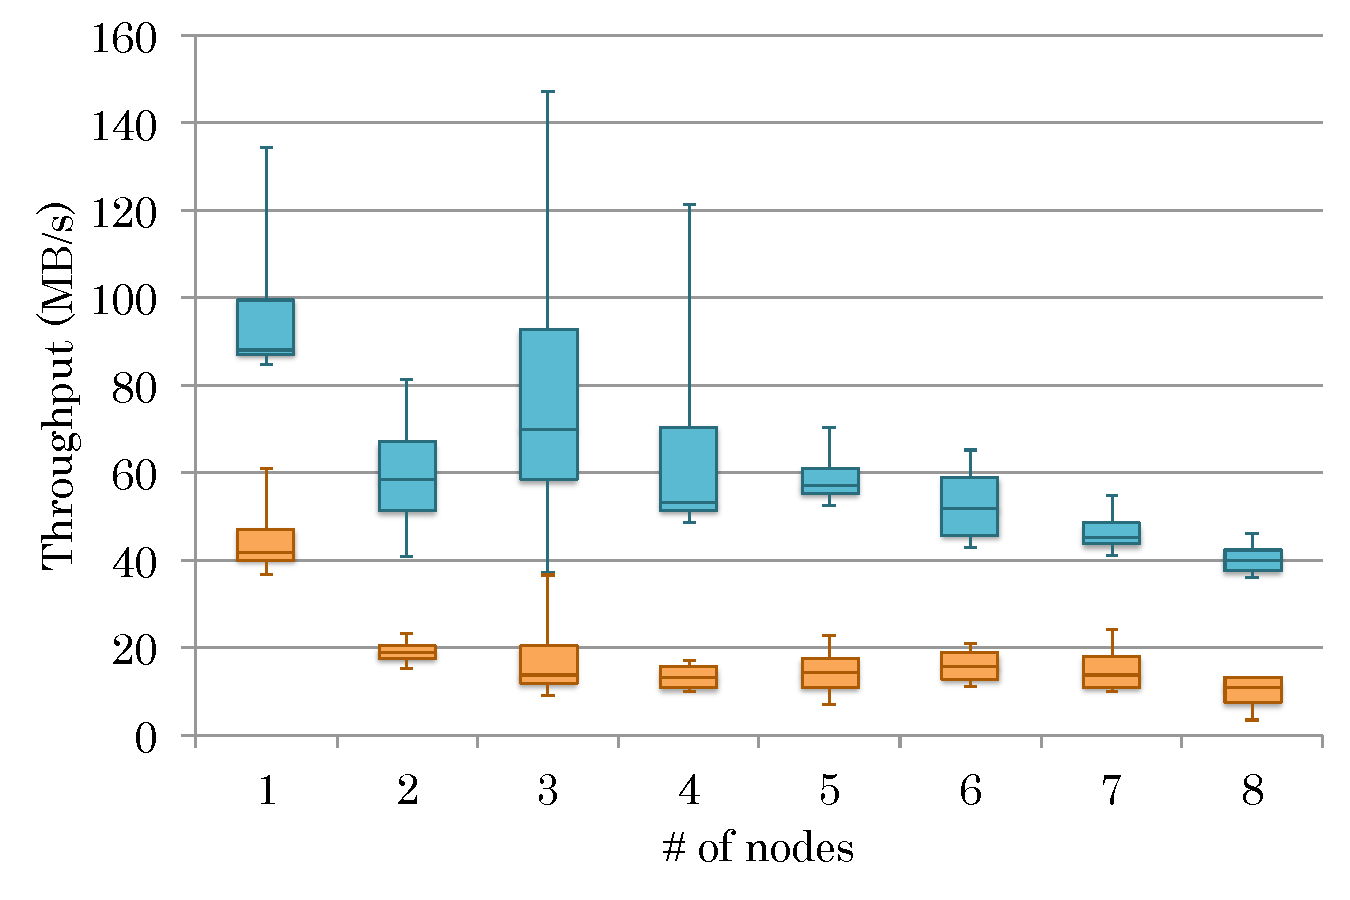
\includegraphics[width=4.1cm]{img/s3_read_write_same_file}}
% % \subfigure[Amazon S3 write (same file)]{
% % \label{background:amazon s3 write same file}
% % 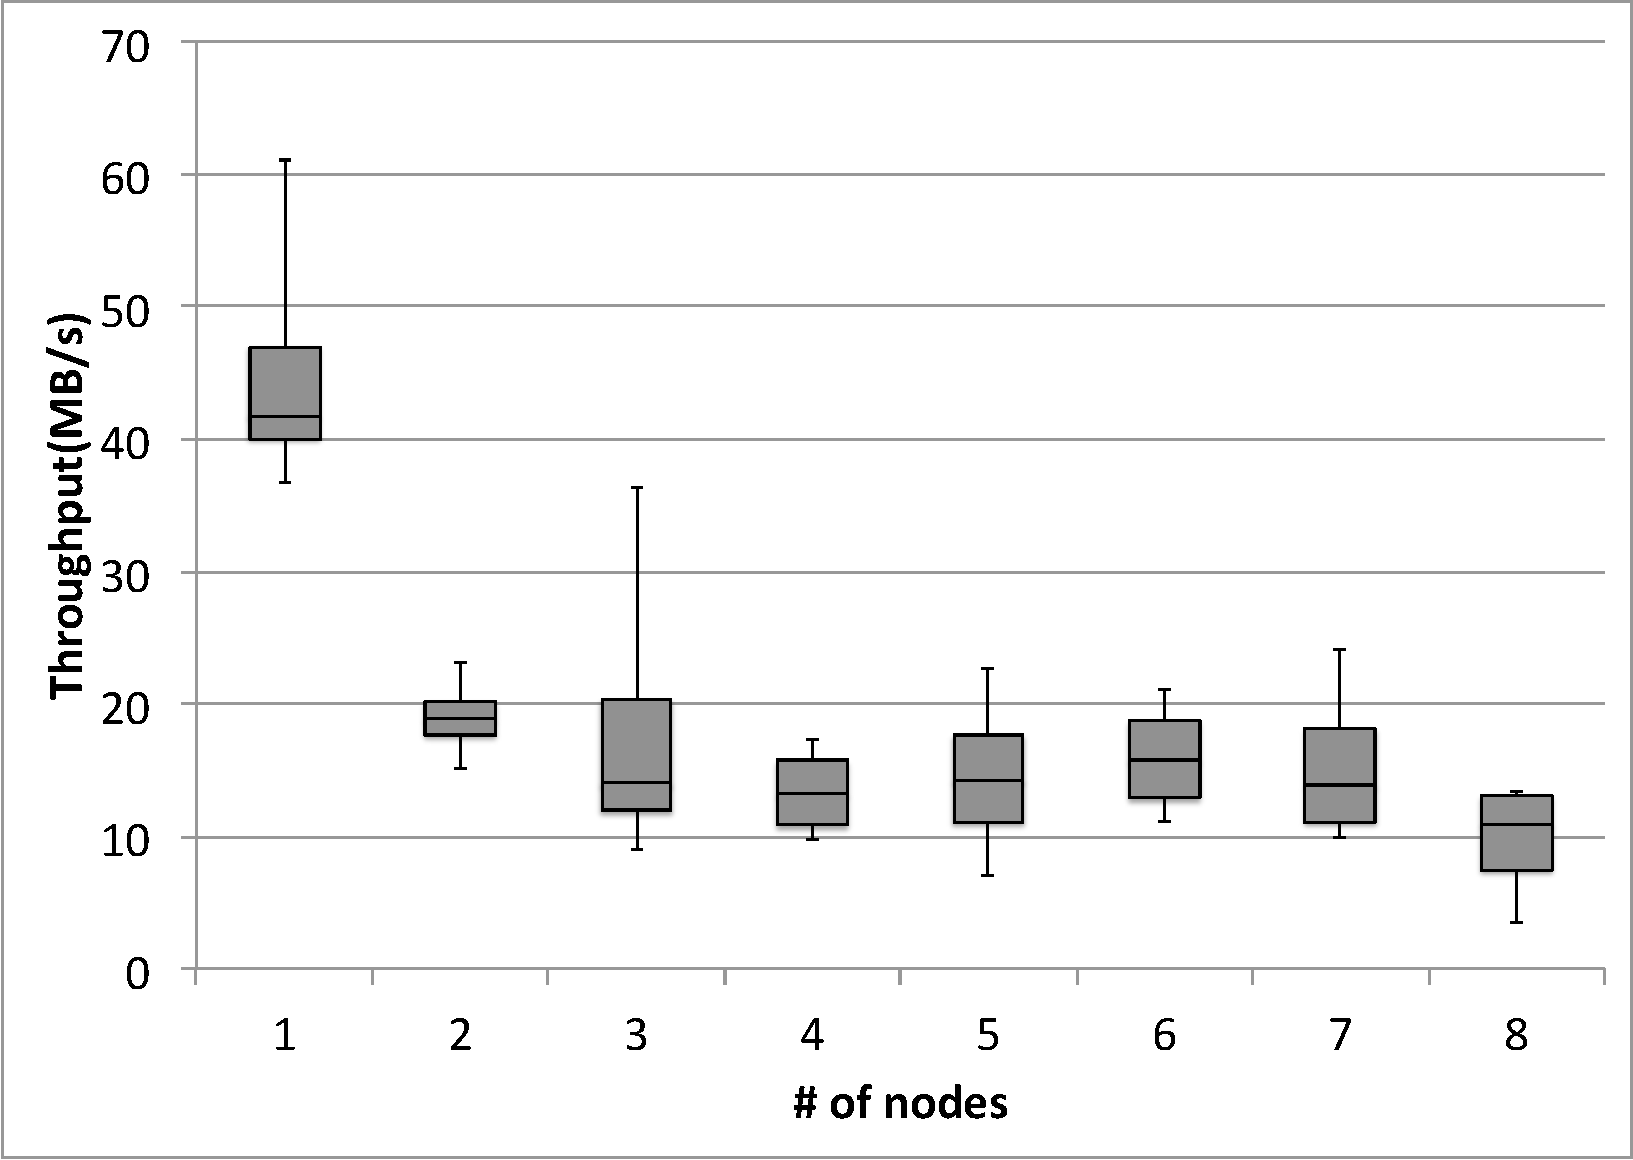
\includegraphics[width=4cm]{img/s3_write_same_file}}
% % \subfigure[Amazon S3 read (different file)]{
% % \label{background:amazon s3 read different file}
% % 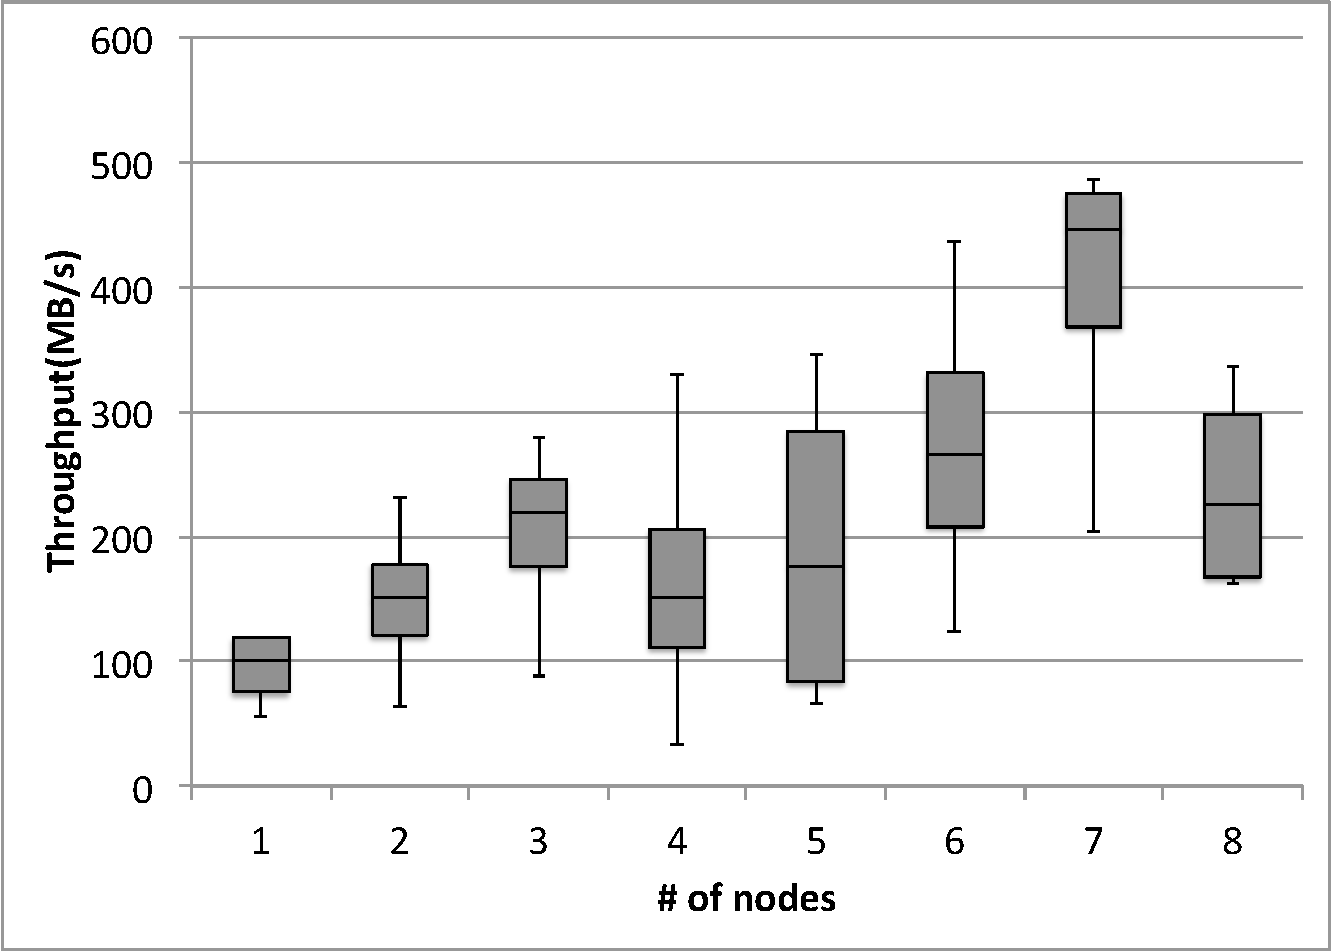
\includegraphics[width=4cm]{img/s3_read_different_file}}
% \subfigure[Amazon S3 read/write (N-N)]{
% \label{background:amazon s3 read write different file}
% 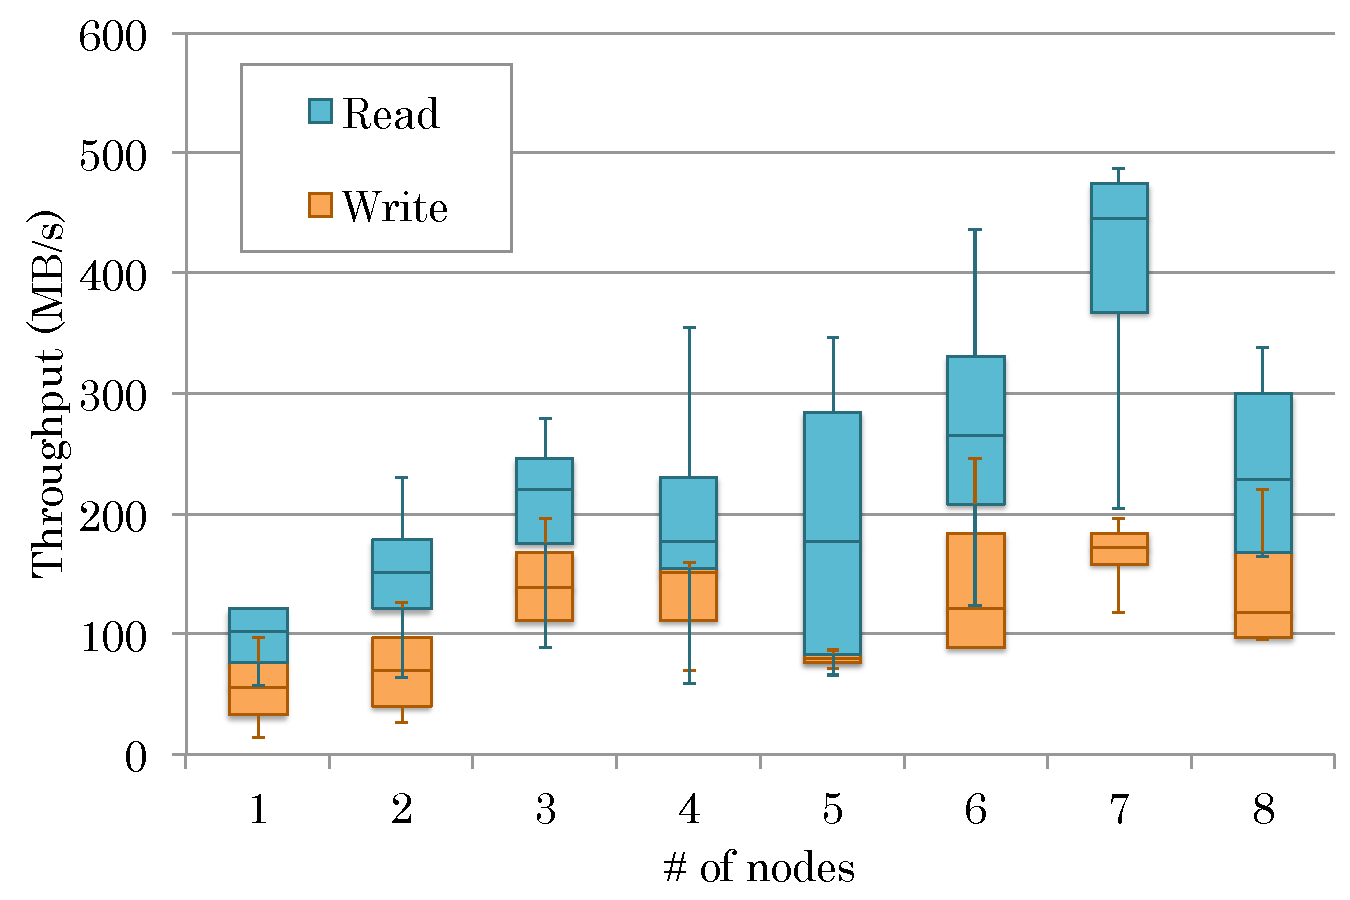
\includegraphics[width=4.1cm]{img/s3_read_write_different_file-2}}
% \caption{Amazon S3 I/O throughput}
% \label{background:amazon s3 throughput}
% \end{figure}
% 

\begin{figure}[t]
\centering

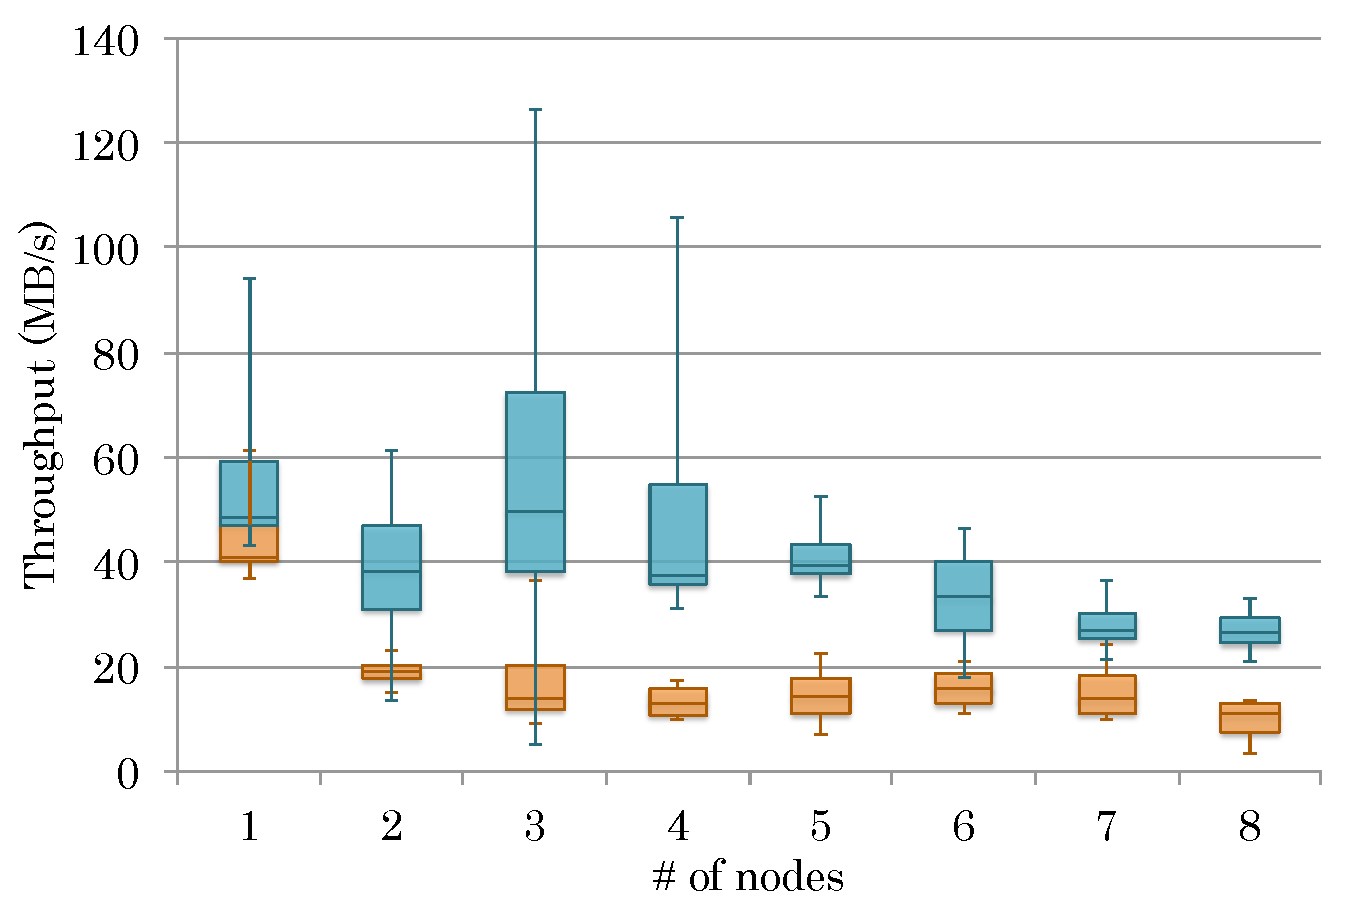
\includegraphics[width=8cm]{img/s3_read_same_file-2}
\caption{Amazon S3 read/write (N-1)}
\label{background:amazon s3 read write same file}
\end{figure}

\begin{figure}[t]
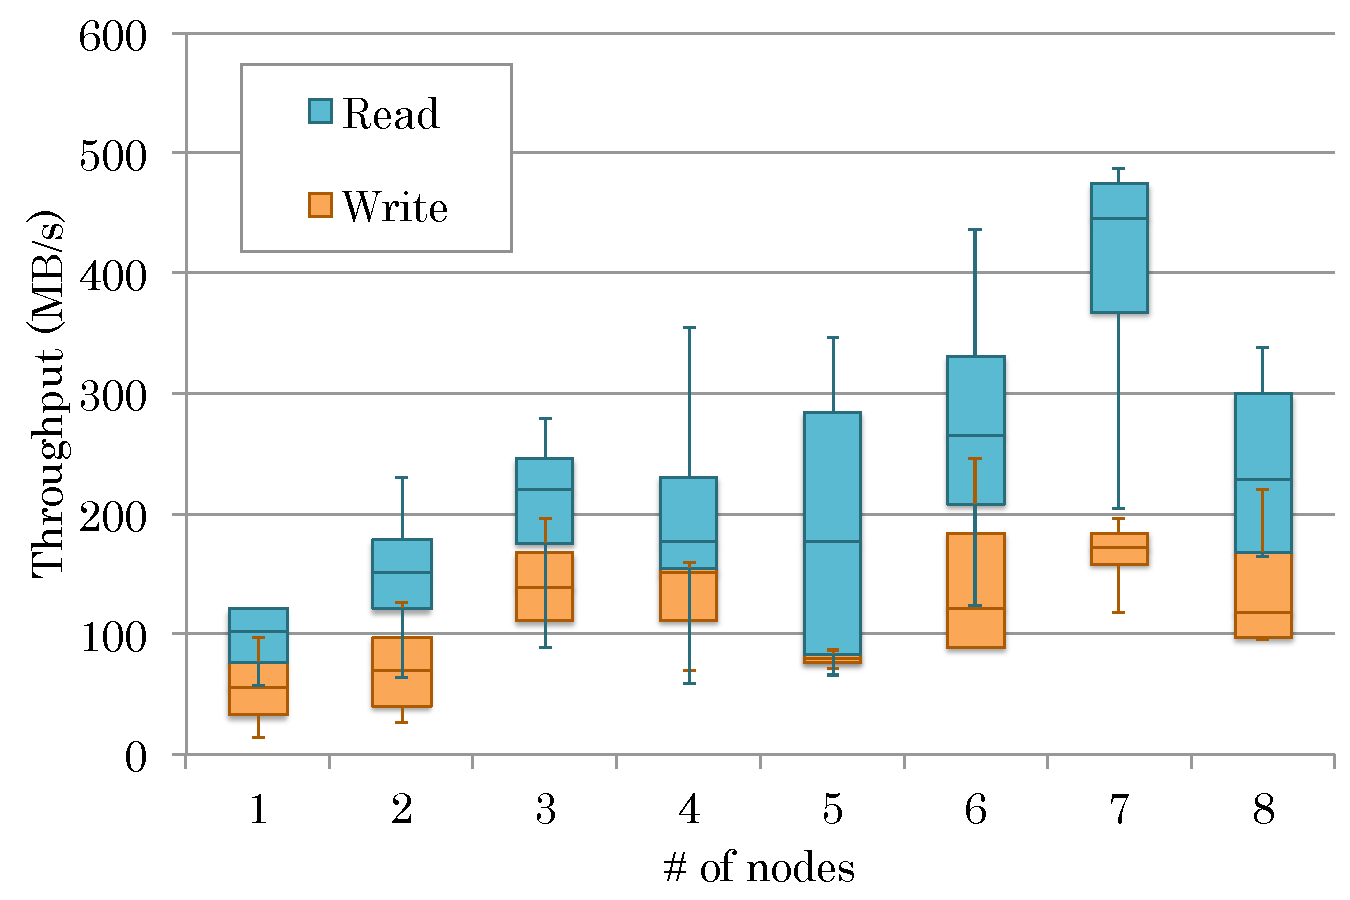
\includegraphics[width=8cm]{img/s3_read_write_different_file-2}
\caption{Amazon S3 I/O throughput (N-N)}
\label{background:amazon s3 read write different file}
\end{figure}



The computational power in clouds enables the users to run high performance
scientific applications faster than ever, which have been making cloud
computing attractive to large scale scientific applications.
However if we run data intensive workloads, which read and write a huge amount
of data, the prolonged execution time can be unacceptable because of the low I/O
throughput in cloud storage.
\par
Figure \ref{background:amazon s3 read write same file} shows I/O throughputs
with different numbers of nodes which read or write to a single file, i.e.,
N-1 I/O.
As shown, the I/O throughputs are only 150 MB/s even in the best case of read,
which degrades performance of data intensive workloads. 
Figure \ref{background:amazon s3 read write different file} shows I/O
throughputs with different numbers of nodes which read or write to their
individual files, i.e., N-N I/O. If each node read or write to their
individual files, we see improvement in scalability compared to N-1 I/O. 
However, the improvement is limited. Especially, write performance does not
scale to the number of nodes. From the figures, we also see that the I/O
performance is fairly unstable. Because typical data intensive applications consist of
processes which have dependency each other, prolonged I/O
operation due to the instability can propagate, and degrades the overall
performance \cite{montage, povray}.
These problems are also reported in several existing studies
 \cite{Chiba,Transactions_a_la_carte, Interactive_Use_of_Cloud_Services,Amazon_S3_for_Science_Grids, anevaluation}. 
Thus, new technology is required to achieve higher and more stable I/O
performance.

 



\subsection{Temporal I/O Locality in Data Intensive Workloads}
\label{ssec:data_access_locality}
\begin{comment}
add other kinds of application data locality details.
as more as possible
\end{comment}

\begin{table}
\centering
\begin{tabular}{|c|p{150pt}|}
\hline
\cellcolor{lightgray} Montage	&
 A portable software toolkit for constructing custom, science-grade mosaics by
 composing multiple astronomical images~\cite{montage}.\\\hline 
\cellcolor{lightgray} POV-Ray   &
 A ray tracing program which generates images
 from a text-based scene description~\cite{povray}.\\\hline
\cellcolor{lightgray} Supernovae &	
 A astronomical program that builds a catalogue of
objects from astronomical images using Source-Extractor\cite{SExtractor}, 
and find supernovae from the images in a CFITSIO data format \cite{fitsio}.
% a library of C and Fortran subroutines for reading and writing data files
%in FITS (Flexible Image Transport System) data format to find supernovae in a
% set of astronomical image.
\\ \hline
\end{tabular}
\caption{Real data intensive workflow applications}
\label{background:work flow applications}
\end{table}

\begin{figure}
\centering
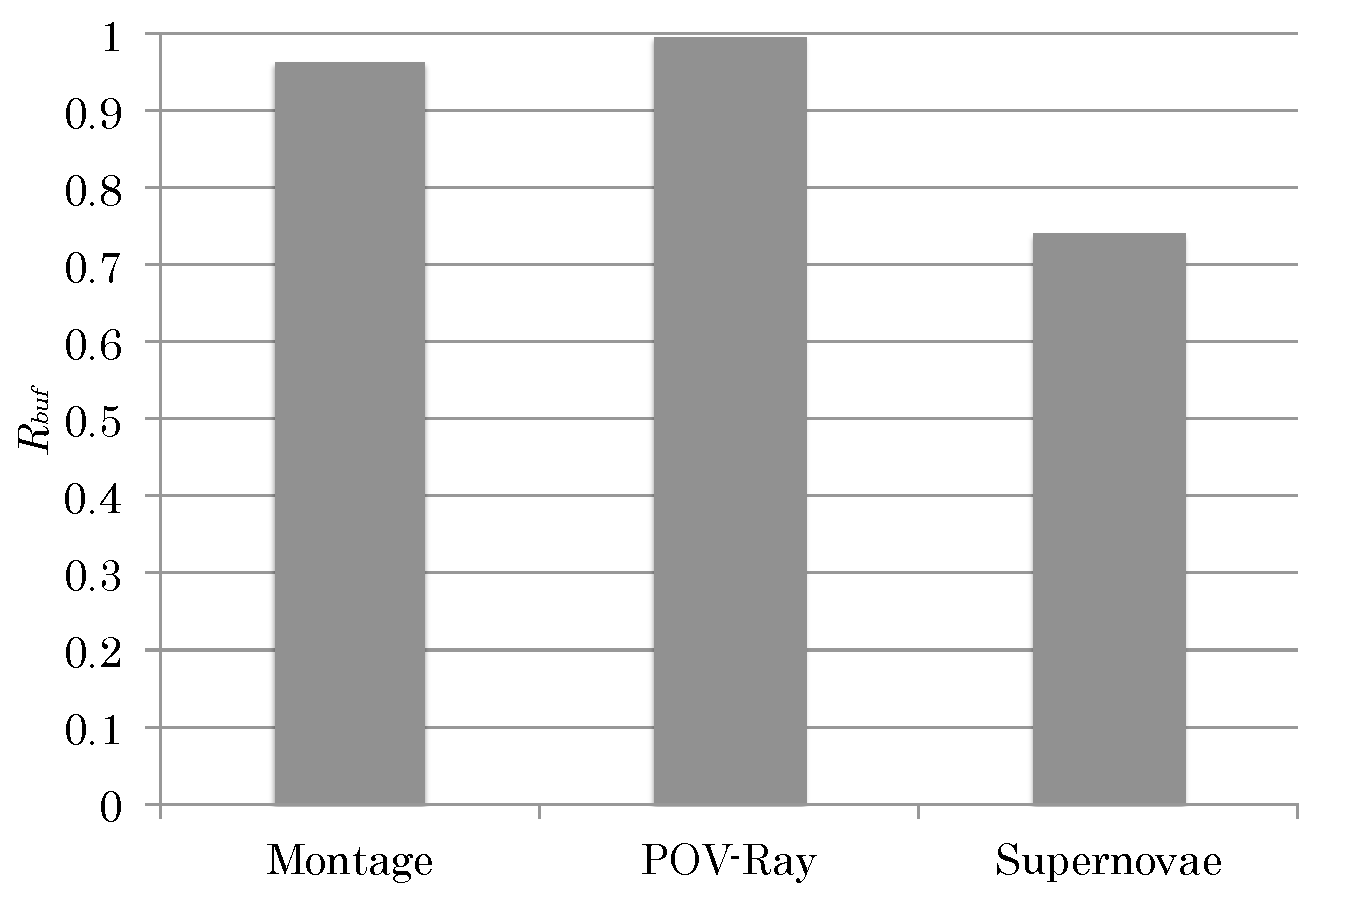
\includegraphics[width=8cm]{img/data_locality-2.pdf}
\caption{Temporal I/O locality in data intensive applications}
\label{background:data locality}
\end{figure}

%\kento{There is no topic sentence in this subse$ction. Why did you write this
%subection ? why do you describe data access locality}
% Since our proposal
% system buffer I/O data and as previous section shows the buffered data can be accessed in a high
% throughput, applications' data access locality will affect the performance gains by using our
% propose system greatly.
% Data locality is a phenomenon describing the same value, or related storage locations, being
% frequently accessed.
% Technology like cache, instruction prefetch for memory, or the advanced
% branch predictor at the pipelining of processors is based on this phenomenon.
% Many previous research investigated data locality of various
% applications including 
% mapreduce,\cite{Investigation_of_Data_Locality_in_MapReduce}, scientific
% \cite{Intrinsic_data_locality_of_modern_scientific_workloads},
% OLTP\cite{Data_locality_characterization_of_OLTP},
% numeric\cite{Analyzing_data_locality_in_numeric_applications}, checkpointing\cite{checkpointing}
% workloads etc., and showed that these applications has a strong data locality.
% \kento{If possible with you, please describe also checkpointing workloads}
% Among these applications, work flow applications shows a strongest data locality, in this paper, we
% focus on work flow applications.
% We measure the I/O data locality for the applications shown in
% Table~.\ref{background:work flow applications}.
% We count the duplicated read at the same position and all write as data locality size, since all
% these cases data can be read from or write to buffer.
% Figure~.\ref{background:data locality} shows the results of these three applications.
% We can see
% that the I/O pattern of all the three applications shows a strong data locality. Montage and Pov ray
% are over 90\% and supernovae achieved over 80\%.
However, our analysis of data intensive workloads on HPC systems, we found that
a number of applications have temporal I/O locality.
To investigate temporal
I/O locality of data intensive workloads,  we run several real data intensive
applications (in Table~\ref{background:work flow applications}) on our in-house
system using MUSE \cite{MUSE}. We devlopped MUSE to trace the all I/O
operations, which include timestamp, pid, types of I/O operations, path to the access
files, offset of file, and the size, so that we can figure out temporal I/O locality of
 data intensive applications from the traced I/O pattern.
Figure \ref{background:data locality} shows the temporal I/O locality in
the different data intensive applications assuming the buffer size is
enough to accommodate the intermediate data.
%\kento{Will change Y. in the figure} 
The buffered I/O ratio, $R_{buf}$, means
ratio of read and write operations, which can read from or write to the buffer.
The ratio can be formulated as:
\begin{equation}
R_{buf} = \frac{r_{b} + w_{b}}{r_{t} + w_{t}} \\
\end{equation}
where $r_{b}$, $w_{b}$ denote total read and write size, and $r_{b}$, $w_{b}$
denote size of reading and writing from the buffer. 
As in the figure, we can see that the I/O patterns of the three applications
shows high buffered I/O rations. For example, The rations of Montage and POV-Ray
are over 95\%, and the ration of Supernovae is over 80\%.
Because we assume enough size of the buffer size, all write operations data can
be buffered, i.e., $w_{b} = w_{t}$.
%\kento{XU: Is this correct ?}
 In addition, the three applications
read all data which is written by another process as intermediate data, which
increases the temporal I/O locality.
\par
 Large scale HPC applications also have high temporal I/O
locality because these applications usually write checkpoints for fault
tolerance. 
In checkpoint/restart, applications read the \emph{lastest} checkpoint when
restarting. The I/O pattern increases temporal I/O locality. 
%\kento{XU: please try to find citation again.}
Thus, improving read and write performance in $r_{b}$, $w_{b}$ can accelerate
these data intensive workloads.


%The reason is that these applications are work flow application, the whole job consists of several
%sub jobs, the output of previous job can be the input of subsequent job, also some job will access
%the same input file.
%So if we buffer the output data and input data, the subsequent job can access the data via LAN.

\subsection{Motivation to Burst Buffer in Clouds}
\label{ssec:network_s3}

\begin{figure}
\centering
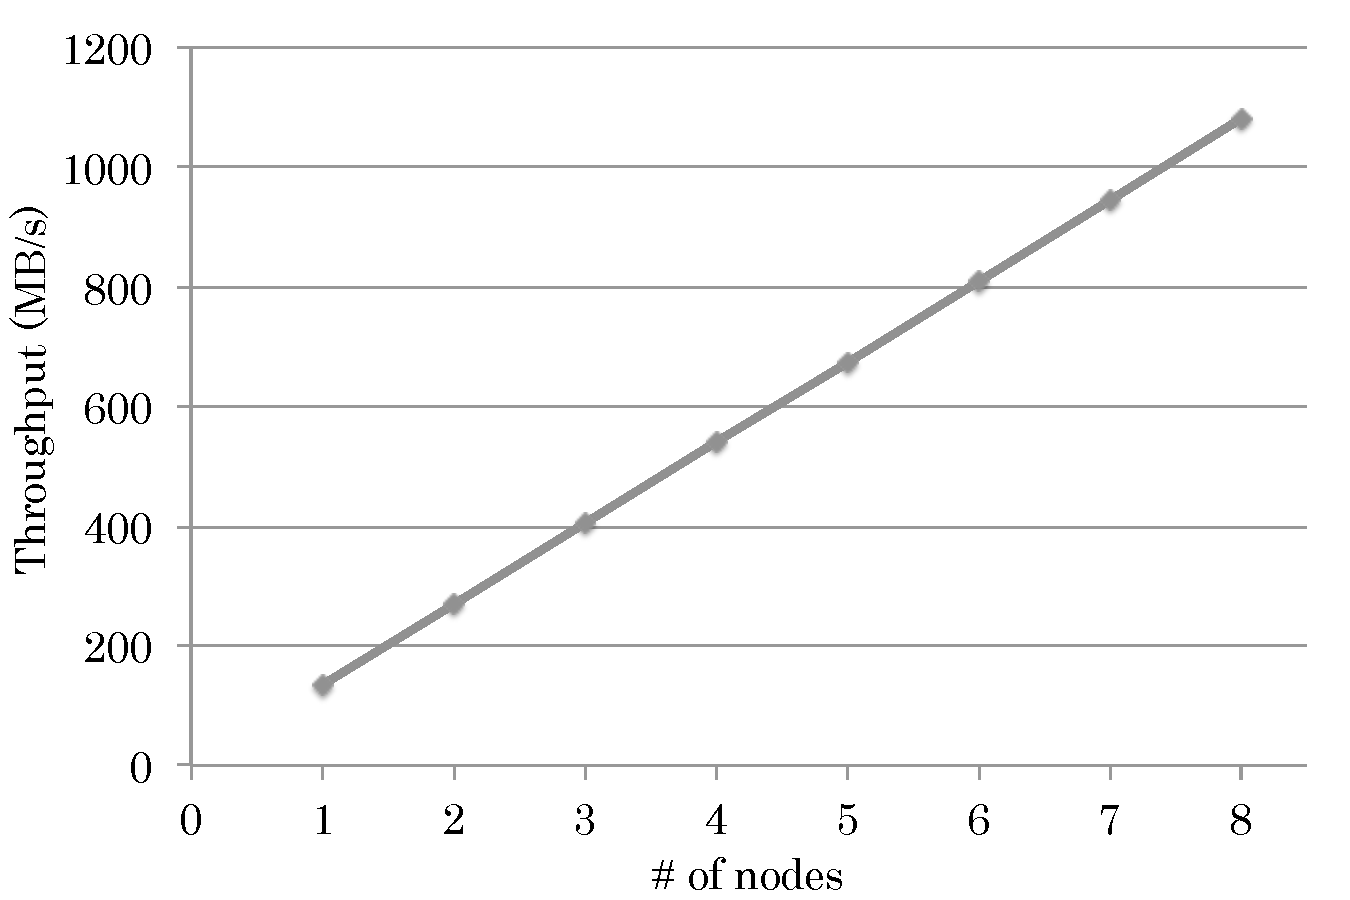
\includegraphics[width=8cm]{img/point_to_point-2}
\caption{Point-to-point communication throughput in Amazon EC2}
\label{background:Amazon point to point throughput}
\end{figure}


% \subsection{Burst Buffer}
% \begin{figure}
% \centering
% 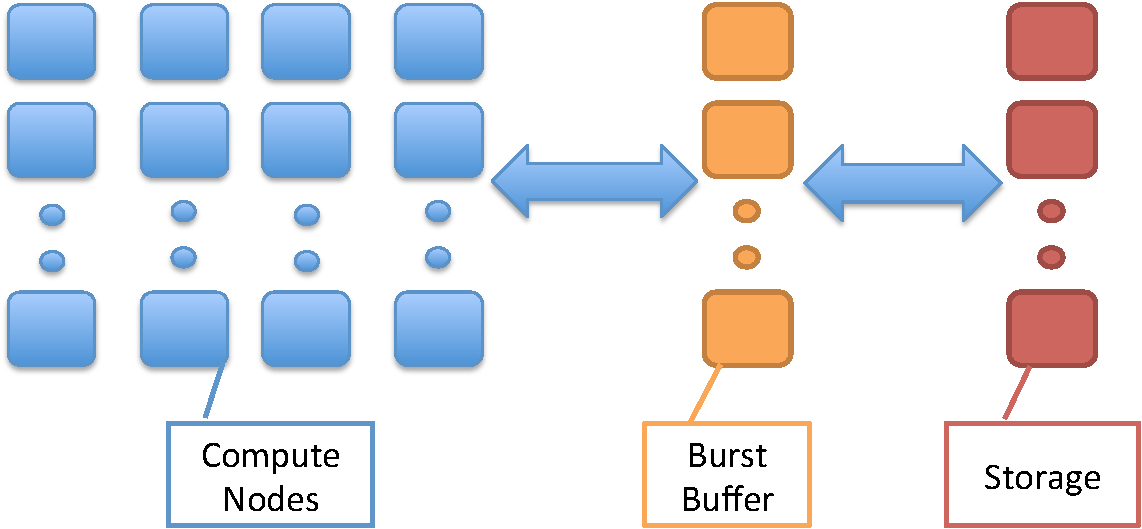
\includegraphics[width=8cm]{img/burst_buffer.pdf}
% \caption{burst buffer architecture}
% \label{background:burst buffer architecture}
% \end{figure}
% 
% Modern high performance systems consist of thousands of compute nodes, and hundreds of
% applications are running at the same time, some I/O request peak can hardly be meet by current
% storage hierarchy. 
% Traditional approach, which solves such problem by providing a higher bandwidth storage will cause
% the storage system under utilization.
% Previous research\cite{on_the_role_of_burst_buffers} proposed a
% burst buffer system as a new tier of current storage hierarchy.
% Burst buffer system uses several local compute nodes as a burst buffer to absorb I/O
% request. 
% By adding such new tier of storage hierarchy, temporal I/O request can be absorb by burst buffer
% without a need of higher bandwidth storage. Figure~.\ref{background:burst buffer architecture}
% shows the architecture of burst buffer.
% 
% Such burst buffer system can burst the application which has a high data locality I/O pattern, since
% the data can be read once from storage and then buffered in the burst buffer system, subsequent
% request for the same data can be accessed from burst buffer.
% Furthermore, applications which write a lot also can benefit from burst buffer system, by buffering
% output data in burst buffer, application can go ahead without waiting data be finally write to
% storage.
% \kento{I think we do not need this subsection or we should combine with the
% previous subsection, because there is no new information from the introduction
% section}


As mentioned in Section \ref{ssec:data_access_locality}, 
a number of data intensive workloads have temporal I/O locality, and their I/O
data can be buffered.
If we can install \emph{large}, \emph{fast} and \emph{shared} buffer space, we
can accelerate these data intensive workloads.
Motivate by the fact, we innovate the \emph{burst buffer} technology to cloud
environments.
Burst buffer is a new tier in current storage hierarchy for bursty I/O operation
in data intensive applications~\cite{on_the_role_of_burst_buffers} and
checkpointing workloads~\cite{A_User-Level_InfiniBand-Based_File_System_and_Checkpoint_Strategy_for_Burst_Buffers}.
By innovating the new tier of storage, the bursty I/O workloads
can be absorbed without a need of higher bandwidth storage.

Figure \ref{background:Amazon point to point throughput} shows Point-to-point
communication throughput in Amazon EC2. In this evaluation,
we measure the network throughput between a pair of $m3.xlarge$ instances using
Iperf~\cite{iperf}, and increase the number of the pairs. The specification of
the instances is in Table \ref{evaluation:amazon_environment}.
As in the figure, we can see that the network throughput between two nodes is
high and scalable to the increasing number of the pairs.
We take advantage of the high and scalable network throughput to burst I/O
throughput. If we use the memory space of bunch of instances as burst
buffers, we can construct on-demand burst buffer with high throughput
and high scalability on the fly.


% However, when we look at the point to point communication throughput between two compute nodes
% inside Amazon EC2,
% We measure this interconnection network by using Iperf [14].
% \kento{What does the ``inside'' mean ? please describe what did you measure}
% Figure.~\ref{background:amazon throughput} shows a comparison of Amazon Interconnection Network
% throughput and Amazon S3 throughput, although we only show the result up to 8 pairs of nodes
% \kento{Because you did not describe how to measure the performance,
% ``pairs'' is not unknown}, each node achieved only 135MB/s (1GBit/s), the
% influence between nodes is extremely small, figure shows a perfect linear line also a strong scalability.
% \kento{It's too detailed. And Should be mentioned before showing results}.
% When we running the
% benchmark, many other users were also running applications on Amazon, so we can assume that highest
% throughput 1GB/s (8Gbit/s) shown in Figure.~\ref{background:amazon throughput} is not the
% maximum bandwidth of interconnection network in Amazon EC2 \kento{Why do you
% mention this ? If you want to say ``this results is not trustful because other
% applications were running'', please remove this figure and this subsection.
% Instead, you should mention ``Even with other applications are running, the
% performance is still better than S3'' . But, in fat tree topology, almost peak
% throughput can be achieved even if other applications are running like in
% TSUBAME. So I do not think your expectation is true}.
% As Figure.~\ref{background:amazon throughput} shows, Interconnection Network throughput inside
% Amazon EC2 is proportional to numbers of nodes used, on the contrary, Amazon S3 throughput is much
% lower than it, and unstable.
% Also we can find that all nodes access to the same file is slower than access to different file,
% it is because Amazon S3 will distribute different file over machines to
% increase I/O throughput, access to the same file will be limited by S3 server machine bandwidth, and will cause connection
% conflict.
% \kento{Please mention ``so what?''. Why did you compare network(interconnection
% network) and storage(S3) ? People will think this comparison is unfair, and no
% meaning unless you mention that. This subsection looks weird to me because this
% section does not have any ``topic sentence'' and ``so what ?'' sentence}
% \subsection{Challenges in Cloud-based Burst Buffers}
% \kento{exploiting network for I/O, multiple applications, limited buffer size}
% \kento{focus is modeling because \ldots}



%section III
\section{Architecture}
\label{sec:architecture}

%\begin
An overview of I/O burst buffer architecture is described in this section.
As we mentioned in the previous section, our model takes advantage of high throughput inside a system, and use buffer queue system in order to increase throughput between two systems.
%Two kinds of buffer are used in our I/O burst buffer architecture, the first one is in client computing node, first buffer user I/O in the same node, another one is in I/O buffer nodes.
The main idea is that some of computing nodes serve as a I/O buffer nodes in each system, for write I/O data, if buffer queue in I/O buffer nodes is not full, data can first be buffered in buffer queue in the same system, and then client can finish write operation without waiting data be finally transferred to storage system.
Actually, since many jobs use multiple nodes work together and the output of some nodes can be the
input of the others, so for most cases, output data will still be buffered in buffer queue until the whole job finished.
As for reading, if that file is stored in the buffer queue, compute nodes can read from I/O nodes through interconnection network.
In other cases (buffer queue is full when issue a write request or requested file is not stored in buffer queue when issue a read request we call it cache miss), an read from or write back operation described below will be executed. 

\subsection{target environment}
First, we introduce our target environment.
we target at common cloud environment like Amazon EC2, which compute node and data center are distributed geographically distributed.

\begin{itemize}
	\item All compute nodes are connected by large bandwidth and interconnection network, note network topology maybe different in each system, so topology is not specified here, interconnection network performance is measured by throughput.
	\item There is a shared storage for date sharing inside system, all compute nodes are connected with shared storage via Internet or other lower network, also the file system of shared storage is not specified and performance is measured by throughput.
\end{itemize}

\subsection{I/O Burst Buffer Architecture}

\begin{figure}[tb]
	\centering
	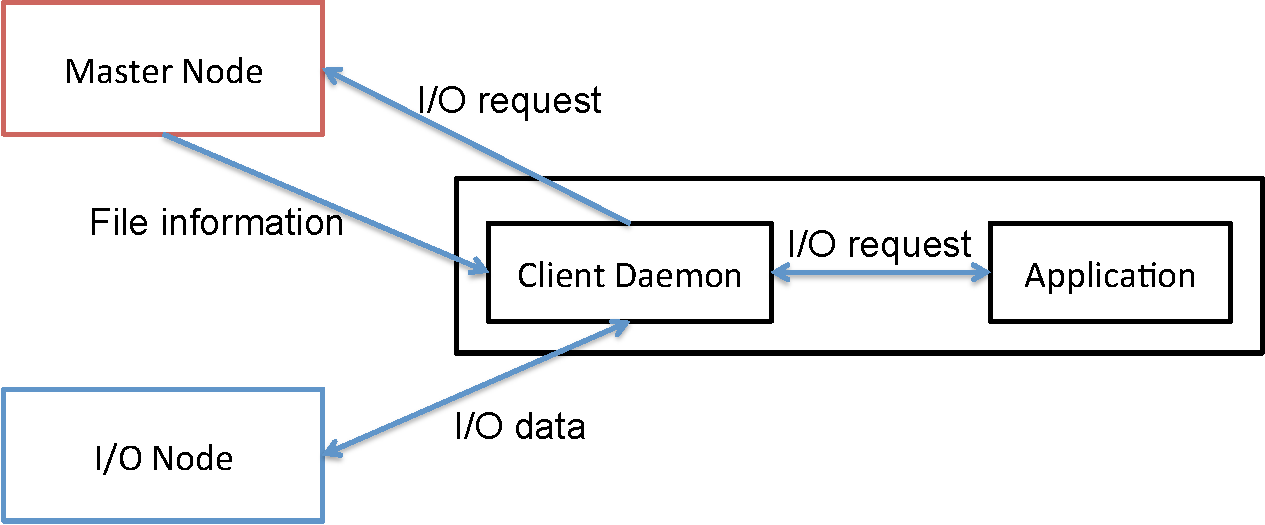
\includegraphics[width=8cm]{img/client_daemon}
	\caption{Client Daemon}
	\label{architecture:client_daemon}
\end{figure}

\begin{figure}[tb]
	\centering
	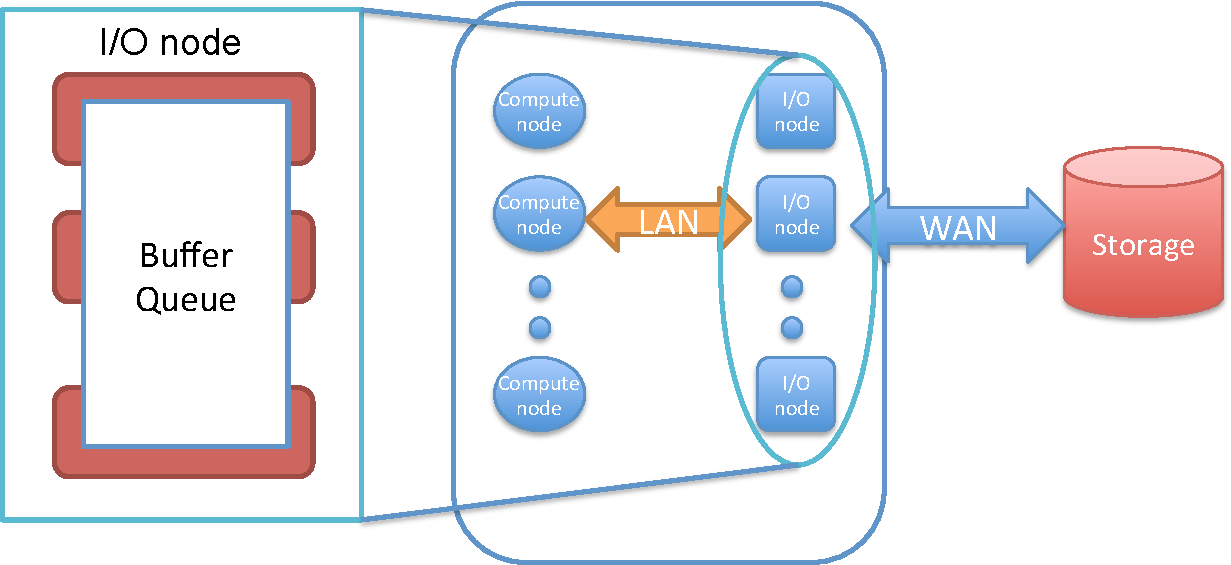
\includegraphics[width=8cm]{img/architecture_overview}
	\caption{overall illustrate of I/O Burst Buffer Architecture}
	\label{architecture:overview}
\end{figure}

There are two kinds of nodes in our I/O burst buffer architecture: \emph{compute nodes} and \emph{I/O burst nodes}, compute nodes run user's application and I/O burst nodes.
Public clouds usually provide several type of instance for difference purpose, some are compute optimized(like C3 instances provided by Amazon) provides a high compute performance,
some are memory optimized (such as R3 instances in Amazon EC2) provide a huge amount of memory(up to 244GB in R3 family), also memory size can be easily expanded by using solid storage driver(SSD) as a swap device, usually such instances have SSD inside.

Fig.~\ref{I/O server} is a illustrate of I/O server inside client nodes and buffer queue in I/O burst nodes.
In each compute node, there is a client daemon, which is a file system client used to buffer I/O data, communicate with I/O buffer nodes, including send I/O request and send or receive I/O data.

When a user application issue a write request, I/O data will be buffered in that node by I/O daemon, when user close the file, call flush function or I/O data size exceed I/O server buffer size, I/O server will try to transfer I/O data to buffer queue in I/O burst buffer, if buffer queue in not full, I/O data will be sent to I/O burst buffer via interconnection network and can be seen among computing nodes in the same system after that.
However if buffer queue is full, I/O server will block user application and wait until buffer queue is ready to receive new I/O data, causing a low I/O throughput.

%When I/O server is notified that buffer queue is ready,first, I/O server sends the size of I/O data to master I/O burst buffer node, master node return a list of several I/O buffer nodes, then I/O server split I/O data into pieces, and sends each pieces to a I/O buffer node, after data transfer finished, that file will be added to buffer queue and namespace, and this file can be seen by all computing nodes, since we assume that all nodes used by the same job are allocated in the same system, so data consistency can be guaranteed since that.
%Buffer queue operation including data write back and operation when queue is full will be described in following section.

Similarly when user issue a read request, there are two conditions: required file is buffered in buffer queue in I/O burst buffer, or file is stored only in storage in another system.
In the first cases, file can be transferred to computing nodes from buffer queue directly, and can achieve a high throughput.
If data is not in buffer queue, then a read operation described below will be executed, since data must be transferred from storage in another system, in this case, throughput will depend on Internet condition and it is hard to achieve a high throughput.

Fig.~\ref{overview} shows a overall illustrate of I/O burst buffer architecture.

%section IV
\section{Design and Implementation of Our Cloud-based Burst Buffer System}
\label{sec:implementation}
% To achieve the challenges, we design and implement our cloud-based burst buffer.
% \kento{Will write more later \ldots}

\subsection{The Role of The Cloud-base Burst Buffers}
\begin{figure}[tb]
	\centering
	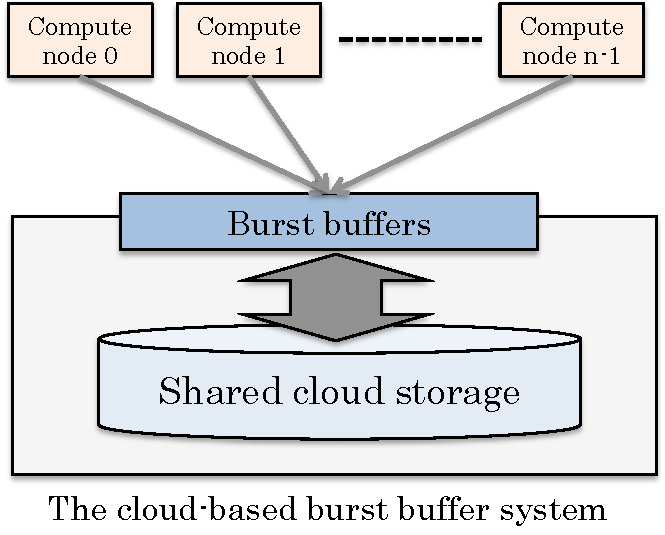
\includegraphics[width=8cm]{img/architecture_overview-2}
	\caption{overall illustrate of I/O Burst Buffer Architecture}
	\label{architecture:overview}
\end{figure}

Figure \ref{architecture:overview} shows an overview of our cloud-based
burst buffer system, which consist of \emph{compute nodes}, \emph{burst buffers}
and a \emph{shared cloud storage}. \emph{Compute nodes} are nodes on which
applications run. \emph{Burst buffers} are provided by the same instances
as \emph{compute nodes}. Unlike \emph{compute nodes}, The instances
of the \emph{burst buffers} provide remote memory buffers for data caching.
When the applications read or write data, the I/O operations are handled via
\emph{burst buffers}.  The \emph{shared cloud storage} is persistent shared storage such as Amazon S3.
Because the applications read or write all data via the burst buffers, the
the caching operations under burst buffers is agnostic to the applications.
Hence, the applications can benefit from the two-level of storage hierarchy
without knowing the underlying operations.

\subsection{Design of The Cloud-base Burst Buffers}
\begin{figure*}
\centering
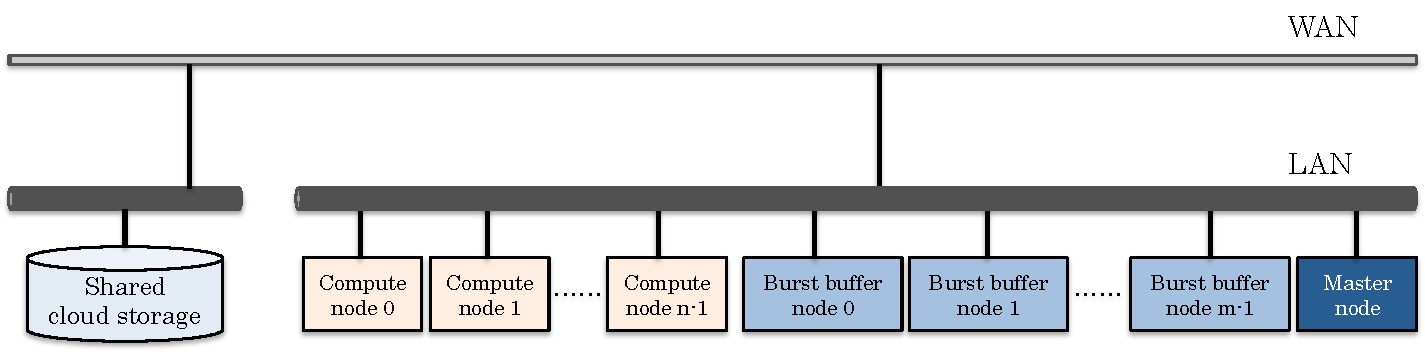
\includegraphics[width=16cm]{img/prototype_overview-2}
\caption{Overview of the prototype}
\label{implemetation:overview of prototype}
\end{figure*}

% In order to validate the effectiveness of the cloud-based burst buffers in real
% environments,  evaluate our architecture in a real environment and compare
% with current architecture, we implemented a prototype.
% Figure \ref{implemetation:overview of prototype} shows the design of cloud-based
% burst buffers.
% In our architecture there are several global data such as total number of burst buffer nodes,
% buffered file information need to be shared between all nodes.
% And since in our proposal architecture, numbers of burst buffer nodes can be dynamically determined,
% a global scheduler is needed to decide when and how nodes are added and removed, these decision
% should be made based on global work load and local work load.
% Also a scheduler is needed to handle the operation like re-balance of buffered data when nodes
% addition, and data write back when nodes deletion.
% 
% For above reasons in this implementation, we adopted master-worker model, a master is designed to
% store global information and interactive with client daemon, as well as serve as a scheduler.
% The architecture of our prototype is described as Figure \ref{implemetation:overview of prototype}
% 
% In our architecture, there are three types of nodes:
% \begin{itemize}
% 	\item A master node manages all burst buffer nodes information, maintains a set of buffered file
% 	meta data, handles operation like burst buffer node addition and deletion etc., and interact with
% 	clients.
% 	\item There are several burst buffer nodes response for actually storing data.
% 	\item A daemon runs on each client machine serving for communication with
% 	master and burst buffer nodes, in order to hide architecture detail from user.
% \end{itemize}
% 
% The shared storage system are mounted on both master and burst buffer nodes,
% both of master and burst buffer nodes have the same assess permission to the shared file system.

In order to validate the effectiveness of the cloud-based burst buffer system in
real environments, we implement a prototype of the system.In our design,
because the number of burst buffer nodes can be dynamically determined, a central management is required to manage when nodes are added and
removed to re-balance the buffered data. In addition, buffered data is
distributed across burst buffer nodes, metadata also needs to be managed by a
control management.For the above reasons, we employ a master-worker model, 
a master is to manage the global information, and handle I/O requests form
compute nodes, and also serve as a scheduler for data placement on burst
buffers.

The architecture of our prototype is illustrated as
Figure~\ref{implemetation:overview of prototype}.
In our architecture, there are three
types of nodes:
\begin{itemize}
	\item Master node: A node managing burst buffer node information for adding and
	removing, maintaining metadata of buffered data, and handling I/O requests
	from compute nodes
	\item Burst buffer node: nodes providing burst buffers using their
	in-memory space
	\item Client daemon: A process running on each compute node, and
	reading or writing data from or to burst buffers based on metadata managed on
	the master node.
\end{itemize}
%The shared storage system are mounted on both master and burst buffer nodes,
% both of master and burst buffer nodes have the same assess permission to the shared file system.

\subsection{File Chunk}
In our implementation, files are usually stored in more than one burst buffer node depends on the files'
size and numbers of burst buffer nodes available.
Files are divided into dynamically determined-size of \emph{chunks} depending
on the sizes of the files, and stored across burst buffer nodes.
% Such one burst buffer node one chunk design simplified our data layout design, and operations in
% burst buffer nodes addition and deletion.
% \kento{I can not understand this. You mean if an application write X bytes
% of data to N of burst buffer nodes, the system divide the data into N of chunks
% with X/N bytes of size, OR totally mutable-size for each chunk ? Please send me
% an email to answer as Q1} \kento{Q2: Given N of burst buffer nodes, can the
% system divide the file into M (< N) ? Please send me an email to answer as Q2} 
Because applications usually generate various sizes of files, data placement
management is important to make use of the memory space.
Since chunk sizes are dynamically determined, our design can avoid
the disadvantage of memory waste in fixed-size chunks, and allocate
memory just needed for buffing data.
%\kento{I can not understand this because of Q1}
% However such one burst buffer node one chunk design and mutable size has some disadvantages.
% First master must maintain the chunk size of each file, this put a burden on master.
% Second, for a large file the chunk size will become very large, cause a coarse-grained write back
% control, and reduce the performance gained by dirty flag.
% \kento{Q3: I can not understand why, because the chunk size is mutable. Please
% send me an email to answer as Q3} Finally, since the chunk size is decided by
% file size, and one burst buffer node store only one chunk, it is difficult to change buffered file size.

Because our cloud-based burst buffer system is served as two-level hierarchical
storage, the system need to manage consistency between files on burst buffers
and shared cloud storage. 
To manage the consistency, we include \emph{dirty flag} in metadata of each
chunk so that modified chunk can be written back to storage.
%This dirty flag can reduce the write back data size and thus reduce the
%Internet congestion.



\subsection{Master Node}
In our master-worker node model, master node is the supervisor of the entire system,
master node is in charge of interactive with client, make file chunk placement, and handle file operations including file open, read and write.
Master node also manages the burst buffer nodes and schedule events like node registration at node
setup phase, addition and deletion.
In order to master node majorly maintains following two data structures:
\begin{itemize}
  \item burst buffer nodes information: including node IP address, total memory and
  available memory. 
  \item File meta data: including file path, file id, total file size, access control, chunk size,
  dirty flag and a map from chunks to burst buffer nodes.
\end{itemize}

Since only master has the global knowledge of file chunk placement, client must connect to master
to get these information.
However, in such master-worker model, master is easy to become a bottleneck of the whole system,
thus we have to minimize the master involvement in file operation, client asks master about the
file meta data, including the chunk placement information, then client uses these information and
connect to burst buffer nodes directly for sending or receiving data.

\subsection{Client daemon}

\begin{figure}[tb]
	\centering
	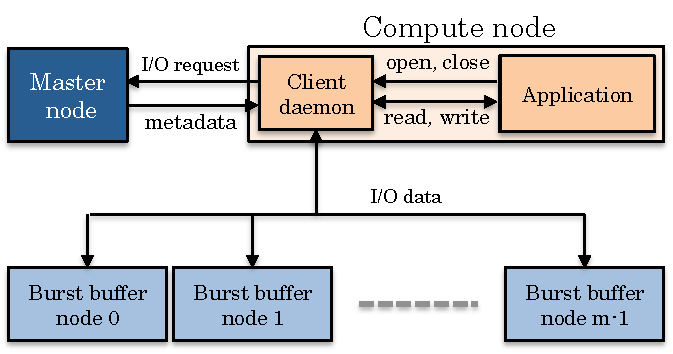
\includegraphics[width=8cm]{img/client_daemon-2}
	\caption{Client Daemon}
	\label{implementaion:client_daemon}
\end{figure}

In each compute node, there is a client daemon, which is a file system client used to buffer I/O
data, communicate with master nodes and burst buffer nodes, including send I/O request and send or
receive I/O data.
Figure.~\ref{implementaion:client_daemon} is an illustration of client daemon inside client nodes
and buffer queue in I/O burst nodes.
Applications changes data with client daemon by using mmap.Figure.~\ref{implementaion:client_daemon}
is an illustration of client daemon inside client nodes and buffer queue in burst buffer nodes.
Users don't know and should not know the information like IP address of master nodes,  client daemon
is used to hide these information from users.
By using client daemon, application doesn't need to change their code, just recompile with a
library.
As figure.~\ref{implementaion:client_daemon} shows, client daemon send open, close request to master
node, and cache the file information including file chunk size, a map to burst buffer nodes.
When applications send read and write request, daemon send the request to corresponding burst buffer nodes
according to the cached information from master node, and transfer data with burst buffer nodes, finally
send to applications.

%When a user application issue a write request, I/O data will be buffered in that node by client
%daemon, when user close the file, call flush function or I/O data size exceed I/O server buffer
%size, client daemon will try to transfer I/O data to buffer queue in I/O burst buffer, if buffer
%queue in not full, I/O data will be sent to I/O burst buffer via interconnection network and can be
% seen among computing nodes in the same system after that.
%However if buffer queue is full, client daemon will block user application and wait until buffer
%queue is ready to receive new I/O data, causing a low I/O throughput.

%Similarly when user issue a read request, there are two conditions: required file is buffered in
% buffer queue in I/O burst buffer, or file is stored only in storage in another system.
%In the first cases, file can be transferred to computing nodes from buffer queue directly, and can
% achieve a high throughput.
%If data is not in buffer queue, then a read operation described below will be executed, since data
% must be transferred from storage in another system, in this case, throughput will depend on Internet condition and it is hard to achieve a high throughput.

\subsection{File Operations}

\begin{figure}
\centering
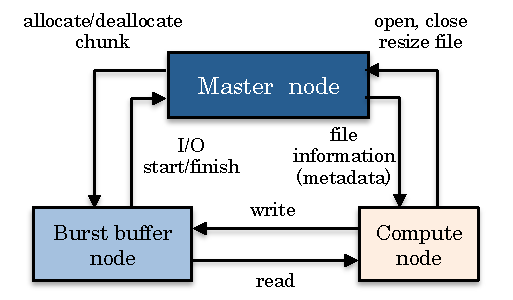
\includegraphics[width=8cm]{img/file_operation-2}
\caption{Details of File Operation}
\label{implementation:file operation}
\end{figure}

In this section we give more details about the file operation in our implementation, including
open, close, read and write.

When an application open a file, client daemon first send file path, access mode to master,
master return the file id,
for unbuffered file, master record the file information, and assign a file id, and then send the
file id to client daemon.

After file opened, applications can use file id to send read or write request.
In our prototype, since the master need to manage the chunk allocate and de-allocate operation, all
the read, write request should send to master.
When master receive the request, for file opened for reading
request for the first time, master get the file size from shared storage, and assign several burst
buffer nodes to this file according to file size and then send a map from chunks to burst buffer
node to client daemon, after that, master connects to corresponding burst buffer nodes, send allocate chunk request and
let burst buffer nodes read data from shared storage.
As for file opened in only writing since the file need to be create, master get file size from
client daemon and assign burst buffer nodes after that master send burst buffer nodes IP address as well as the map
information from chunks to burst buffer nodes to client daemon, then master connects to
corresponding burst buffer nodes, send allocate chunk request.

After receiving the map from chunks to burst buffer nodes, client daemon connect to each burst
buffer nodes in the map, and start I/O with these burst buffer nodes.

In order to monitor workload of each burst buffer nodes, and make load balanced, burst buffer nodes send a signal to
master at the start and the end of each data transfer.

% \subsection{Limitation}
% 
% Since this is a prototype of our proposal system, there are several limitations.
% First, in this prototype implementation, both master node and burst buffer nodes use one thread, it means
% there is only one request can be responded at any time.
% this design may cause master easily becoming a bottleneck when the number of client increase.
% Also, since at any time one burst buffer node can transfer data with only one client, when the bandwidth of
% burst buffer node larger than compute node, it will cause the burst buffer node under utilization.
% However, there are some difficulties to change to a multiple threads version, for example, there
% is a dependency between read from shared storage and send to compute nodes request, burst buffer nodes should
% block the reading request from compute nodes until the read from shared storage finished also
% synchronization is needed among read and write operations.
% 
% Second, one burst buffer node one data chunk design simplified master's design, but it also brings several
% limitations. It is difficult to change the file size after buffered it, as well as it reduce the
% benefit gain by using dirty flag.
% 
% Third, in the node addition and deletion, there is no load balance in our prototype.
% Without load balance, after node added into the system, it needs a long time to achieve speed up.
% Also in the node deletion, file write back and re-buffer are required.
% 
% In this paper, our aim is to validate effectiveness of burst buffers in
% cloud.
% Although we have these limitation in prototype, we can still show the effectiveness of burst
% buffers.

%section V
\section{evaluation}
\label{sec:evaluation}

In this section we introduce the evaluation result of our prototype implementation in Amazon EC2 public cloud.
The cloud environment is shown as Table.\ref{evaluation:amazon_environment}
\begin{table}[h]
\centering
\begin{tabular}{|c|c|}
Region				&		Tokyo		\\
Instance Type		&		m3.xlarge	\\
vCPUs				&		4			\\
ECUs				&		13			\\
Memory				&		15GiB		\\
Instance Storage	&		2*40GB(SSD)	\\
Network Performance	&		High		\\
\end{tabular}
\caption{evaluation environment}
\label{evaluation:amazon_environment}
\end{table}

\begin{table}[th]
\centering
\begin{tabular}{|c|p{150pt}|}
\hline
CPU					&		Intel\textregistered Core\texttrademark i7-3770K CPU @ 3.50GHz\\\hline
Memory				&		16GB\\\hline
Storage				&		Crucial m4 CT256M4SSD3 (256GB, mSATA)(Peak read: 500 MB/s, Peak write:260MB/s)*8\\\hline
RAID Card 			&		Adaptec ASR-7805Q Single\\\hline
RAID				&		Raid 0\\
\hline
\end{tabular}
\caption{stroage environment}
\label{evaluation:stroage_environment}
\end{table}

here vCPUs means the number of virtual CPU in instance, and one ECU provides the equivalent CPU capacity of a 1.0-1.2GHz 2007 Opteron or 2007 Xeon processor.

For the storage system, we used a machine inside our lab, the details is shows in
Table.~\ref{evaluation:stroage_environment}.

All the compute nodes, I/O nodes and master node connect with interconnection network inside Amazon
EC2, and mount storage system by sshfs\cite{sshfs} via Internet.

\subsection{One User Performance}

\begin{figure}
\centering
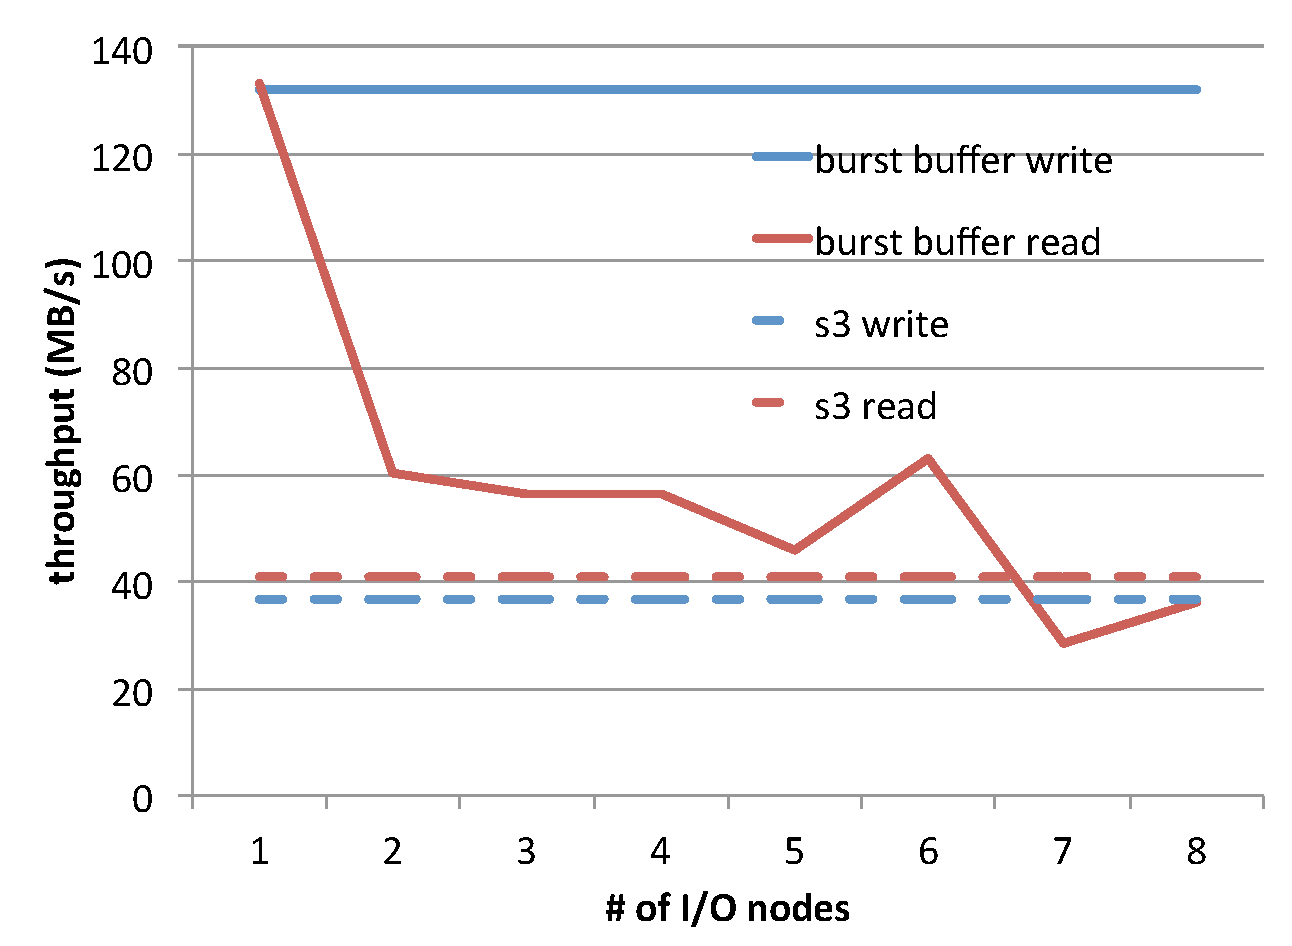
\includegraphics[width=8.5cm]{img/one_client.pdf}
\caption{One User Performance}
\label{evaluation:one user performance}
\end{figure}

First we measure the performance of our prototype for only one user, and shows how our system
will affect one user performance.
In this experiment, the number of client is fixed to one, and measure
the sequential read and write performance for different number of I/O nodes.
All I/O data are distributed among all I/O nodes.
Figure~.\ref{evaluation:one user performance} shows one user performance.
As we know, one thread I/O is difficult to achieve the full throughput on Internet, we can see from
Figure.~\ref{evaluation:one user performance} that without I/O node, applications can only achieve a
throughput under 20MB/s in reading and under 80MB/s in writing.

However by using our system the read throughput increasing as the number of I/O nodes, and can
achieve about 8 times faster than the throughput without I/O nodes.
For writing throughput, the interconnection throughput is different from Internet throughput, it can
achieve full throughput even with one thread, but the throughput is limited by the client node
throughput which is also 1Gbps(135MB/s).

\subsection{Multiple Users Performance}

\begin{figure}
\centering
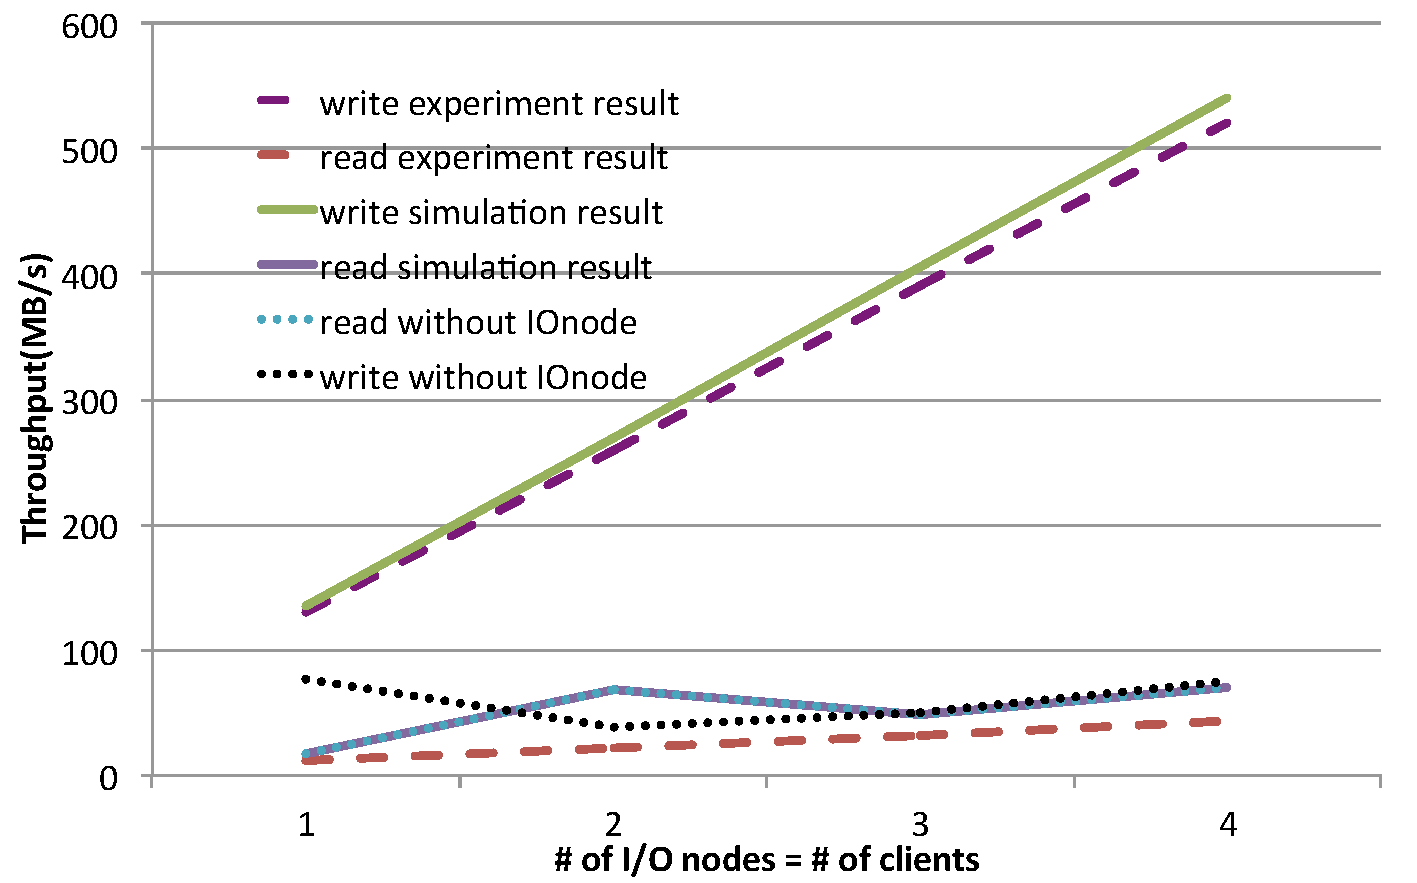
\includegraphics[width=8cm]{img/multiple_client.pdf}
\caption{Multiple User Performance}
\label{evaluation:multiple user performance}
\end{figure}

In the second experiment, we measured the throughput of multiple clients.
To simplified the experiment, we assume that one client connect to only one I/O nodes, and one I/O
nodes buffer all the I/O data for a client.
Figure.~\ref{evaluation:multiple user performance} shows the overall throughput of the whole system.
Since all the data are stored on the shared storage, and need to be transferred via Internet, the
read throughput doesn't change by using I/O nodes.
However when we look at the write throughput, it shows a strong scalability, and achieved 7 times
improvement with only 4 I/O nodes.

\subsection{Simulation for Applications}
Show our architecture can burst I/O performance for applications
x

%section VI
%to do 
\section{related work}
\label{sec:related work}

section VI:related work


%section VII
%to do
\section{conclusion and future work}
\label{sec:conclusion}
In this paper, we propose a cloud based burst buffer system to burst the I/O throughput in cloud.
We implement a prototype of our proposal system, and evaluate it on Amazon EC2/S3 public cloud.
We achieve an up to 3 times speed up for a single user in reading, as well as 4 times speed
up for the whole system in writing.
We also simulate the execution of three real data intensive applications on our proposal system in
a real environment, and achieved up to 1.5 times speed up in the execution time of real application.

However since this is a prototype of our proposal system, there are still many limitation in the
system, may leading to under utilization of node bandwidth, and master node may easily become the
bottleneck of the whole system.
Also there are many points can be improved and can be added to the implementation, including the
data layout of the I/O node in order to make load balance, and dynamic load balance in node addition
and deletion.
For the future work, we will try to improve our prototype.


\section*{Acknowledgement}
This research made use of Montage, funded by the National Aeronautics and Space Administration's
Earth Science Technology Office, Computation Technologies Project, under Cooperative Agreement Number NCC5-626 between NASA and the California Institute of Technology. Montage is maintained by the NASA/IPAC Infrared Science Archive.
\bibliography{src/ref/reference.bib}

\end{document}
